% ************************************************************************
%
% Introduction
%
% ************************************************************************
\chpos{22mm}{10mm}
\chapter[Introduction]{Introduction}
\markboth{\thechapter\ \ Introduction}{\thechapter\ \ Introduction}
\label{ch1:introduction}

%\mysquote{0.8\textwidth}{Quote text.}{Author (\oldstylenums{1000} - \oldstylenums{1100})}

% ************************************************************************
\section{Neuron cell reconstruction} 
Fascination with the neuron cells dates to the time of the first glance into the sample of the neuronal tissue over a century ago \cite{ramon2008histologia}. Eversince the discovery, and the early hand drawings of the magnified images of the neuronal sample, numerous scientists and researchers with various backgrounds and interests have been trying to gain a better insight into the nervous system and the captivating brain mechanism. Numerous technical obstacles stand out when reaching out to the this vast unknown world, primarily due to the physical inaccessibility. The estimated number of neuron cells in a human brain amounts to 89 billion, number comparable to the total count of stars in the Milky Way galaxy. Each is further connected to 50 thousand other neurons on average which results in a very  computational and storage 

Neuron cells represent a core building block of the brain and the nervous system. 

Captivating mechanism of the brain is an everlasting research topic as the complex functionality of the brain . Discovering how the brain works is central to diverse fields such as physics, mathematics, biology and, recently informatics.

Quantification of the neuronal structure is crucial in neuroscience studies \cite{halavi2012digital}. Neuron reconstruction from microscopic images is identified as one of the major technical challenges in the digital era of neuroscience \cite{peng2015diadem}.

The insights in
\begin{figure}
	\begin{center}
		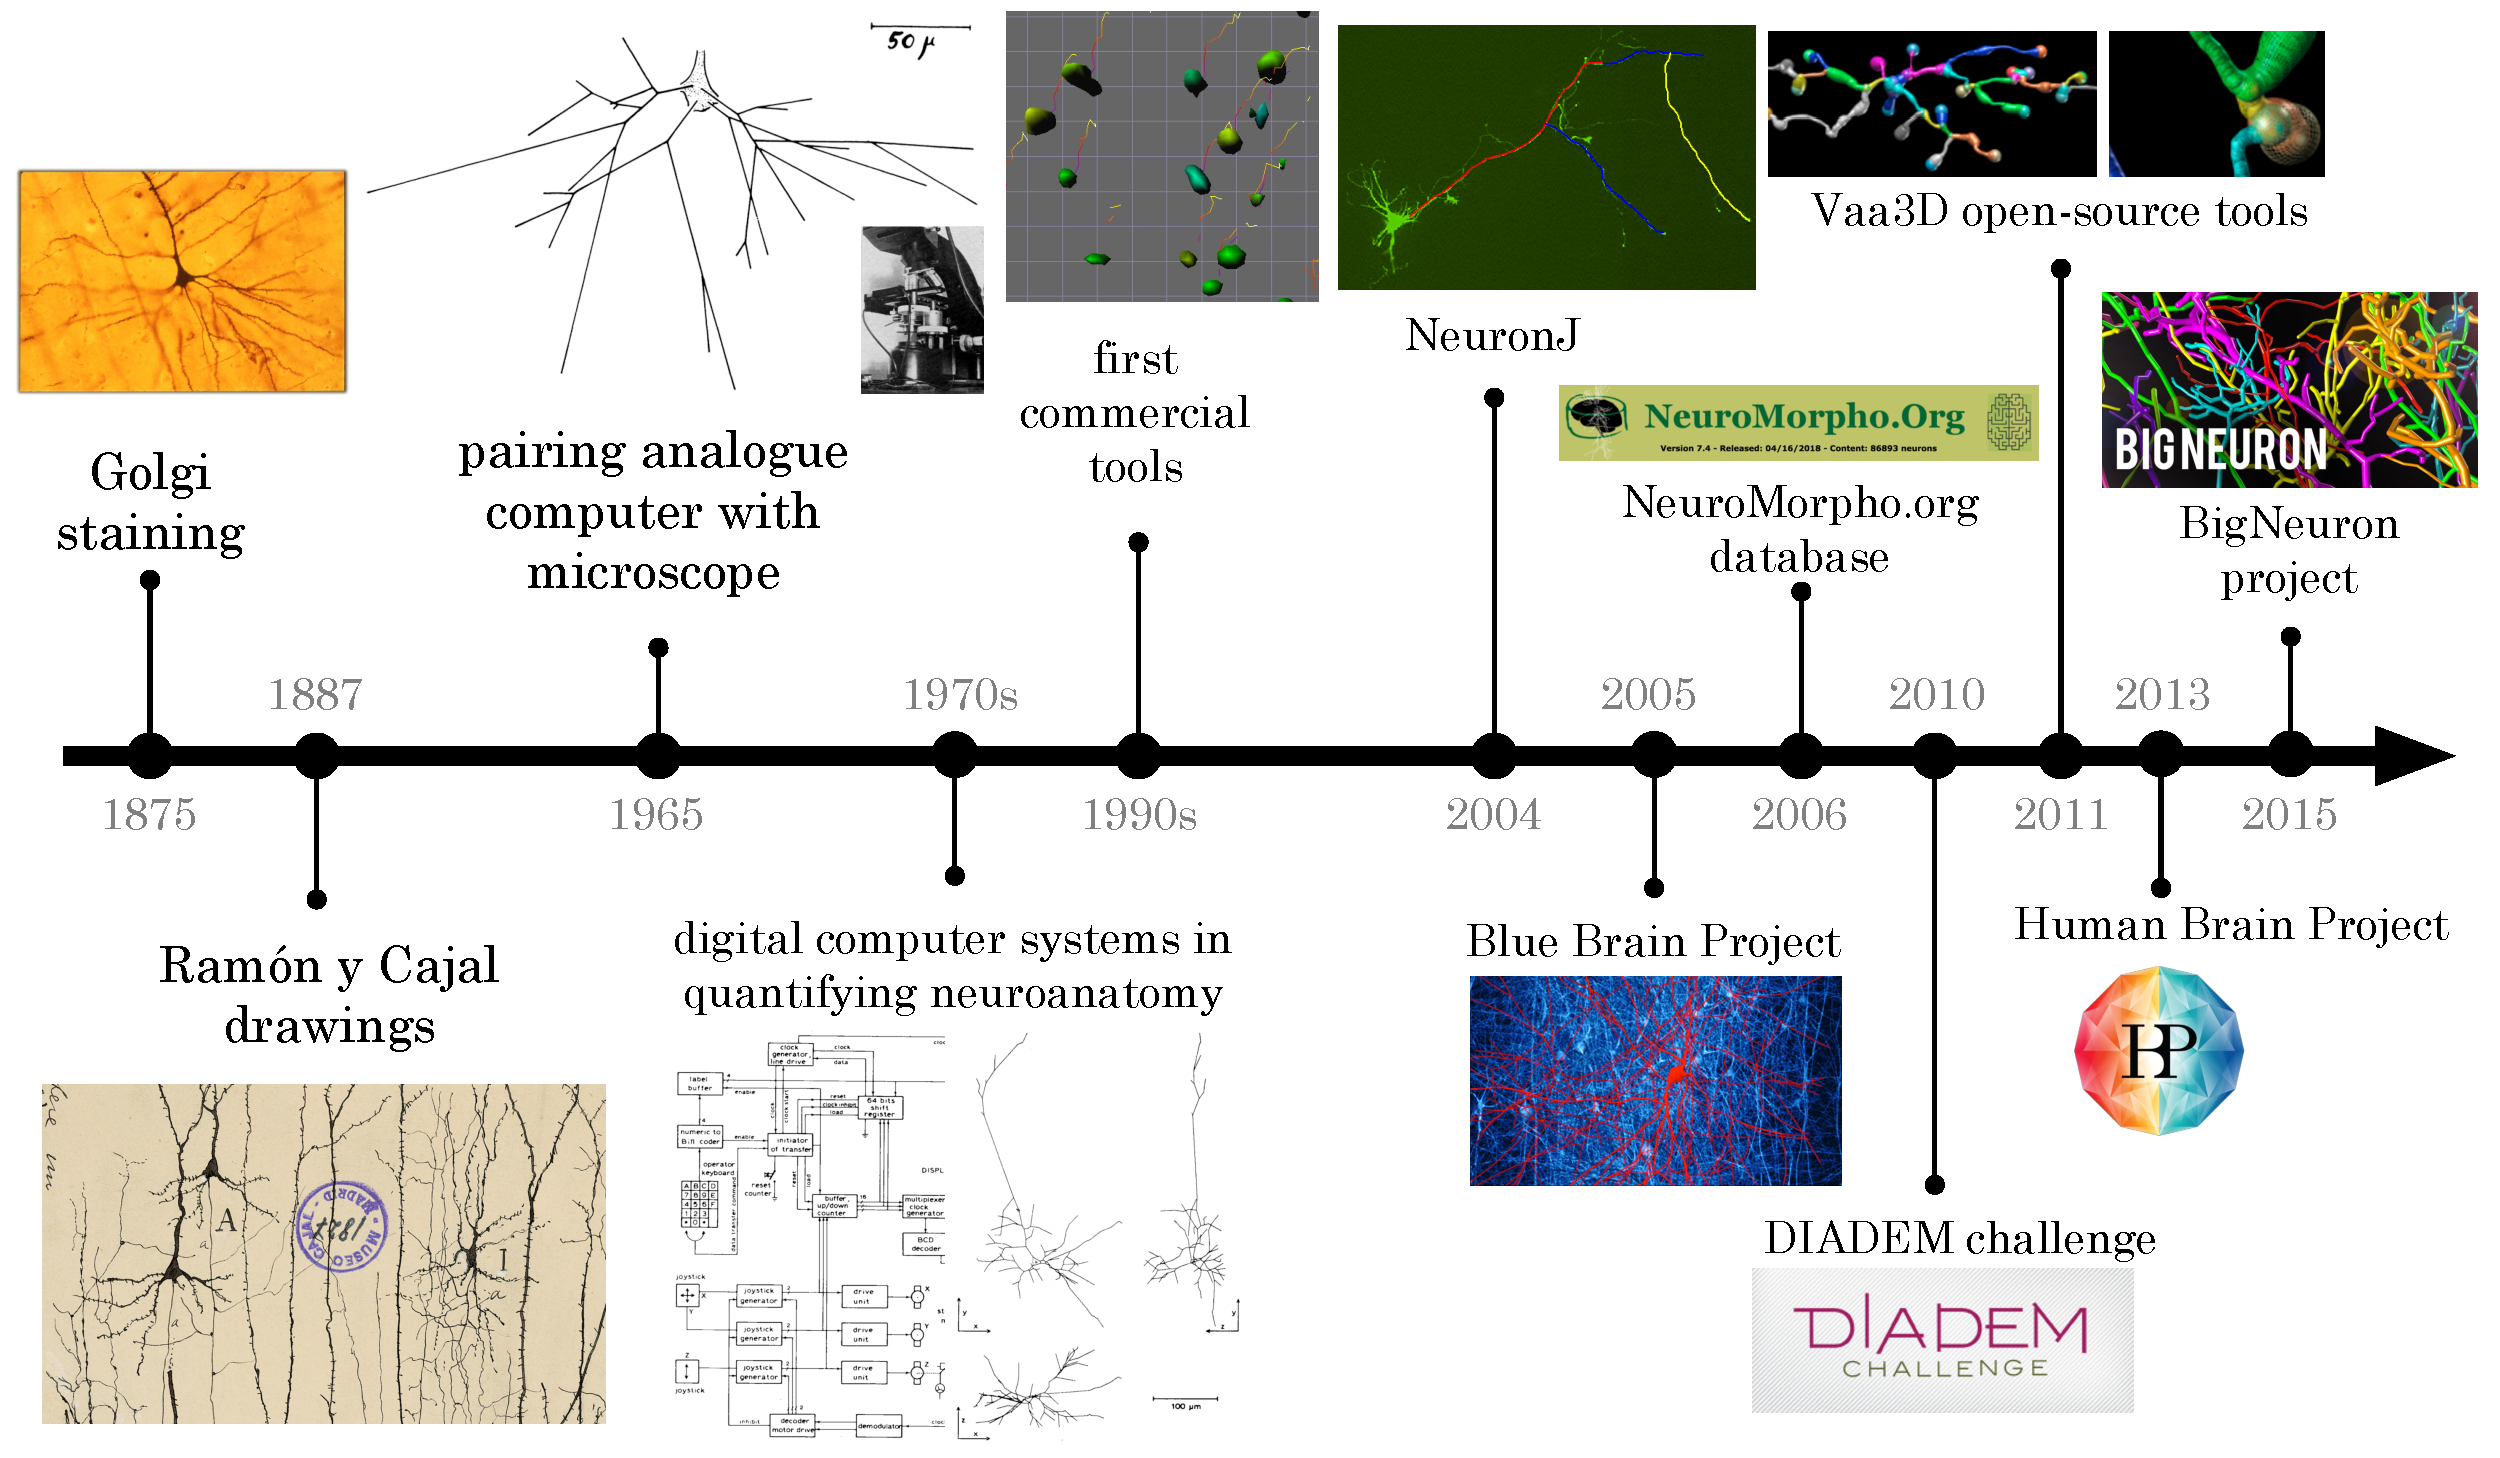
\includegraphics[width=\textwidth]{ch1_fig1}
	\end{center}
	\vspace{-3ex}
	\caption{Neuron reconstruction timeline.}
	\vspace{-1ex}
	\label{ch1__fig1}
\end{figure}

\section{Essential obstacles in neuron reconstruction}

Figure ~\ref{ch1__fig1} represents a neuron reconstruction timeline summary. Several survey publications \cite{meijering2010neuron,donohue2011automated,acciai2016automated}

Microscopic images are capable of .

\section{Tools: notable strategies}
One of the key Java tools is the ImageJ library \cite{abramoff2004image}. 

\begin{figure}
\begin{center}
\includegraphics[width=0.5\textwidth]{ch1_fig2}\\
a) Shortest path tracing \\
\includegraphics[width=0.5\textwidth]{ch1_fig3}\\
b) Minimum spanning tree \\
\includegraphics[width=0.5\textwidth]{ch1_fig4}\\
c) Path-prunning
\end{center}
\vspace{-3ex}
\caption{Examples of key neuron reconstruction strategies: a) Finding optimal path between two fixed points, b) Inferring the  optimal tree structure from the given nodes c) Prunning the overcomplete neuron tree.}
\vspace{-1ex}
\label{ch1__fig2-4}
\end{figure}

Computation methods

\section{Examining the neuronal reconstructions}
SWC format is the .

\begin{figure}
	\begin{center}
		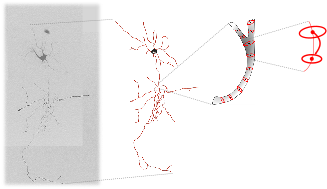
\includegraphics[width=\textwidth]{ch1_fig5}
	\end{center}
	\vspace{-3ex}
	\caption{SWC format of the digital reconstruction, Stockley, Wheal and Cole \cite{stockley1993system}. Visualization using Vaa3D \cite{peng2010automatic}}
	\vspace{-1ex}
	\label{ch1__fig5}
\end{figure}

Distances between neurons can be based on the overlap and the inter-node metric distances.

\section{Thesis outline}
In this thesis.
